\title{Confounders: Protein Length}
\author{Romain Strock}
\date{\today}

\documentclass[12pt]{article}
\usepackage{amsmath}
\usepackage{mathrsfs}
\usepackage{graphicx}
\usepackage{booktabs}
\usepackage[svgnames,table]{xcolor}
\usepackage{pifont}
\usepackage{hyperref}

\graphicspath{ {./figures/} }

\begin{document}
\maketitle

\begin{abstract}
Proteins made of more amino acids have intuitively more chance of closely following their proteome amino acid distribution. We set out to understand whether this relationship between length and distance to mean could partly or fully explain the large number of tRNA synthetase domains in the top of our result set. I found that the relationship between length and distance is quite striking and that proteins appearing at the top of our analysis tend to have a slightly larger size than average. However, when comparing goodness of fit of the length model for the top results versus a control group, it is clear that length alone is not nearly good enough to predict the low average distance of proteins such as tRNA synthetases. I'm able to conclude that length is not a meaningful confounders for our analysis.
\end{abstract}

\section{Length vs distance to proteome mean}

Figure~\ref{fig:length_vs_distance} shows the relationship between protein length and Jensen-Shannon distance to the proteome mean for two organisms. The right column shows the same relationship in log-log scale. This figures makes it very clear that, as intuited, larger proteins have a distribution of nucloetide close to that of their proteome.

\pagebreak

\begin{figure}[!htb]
\hspace*{-1.6cm}
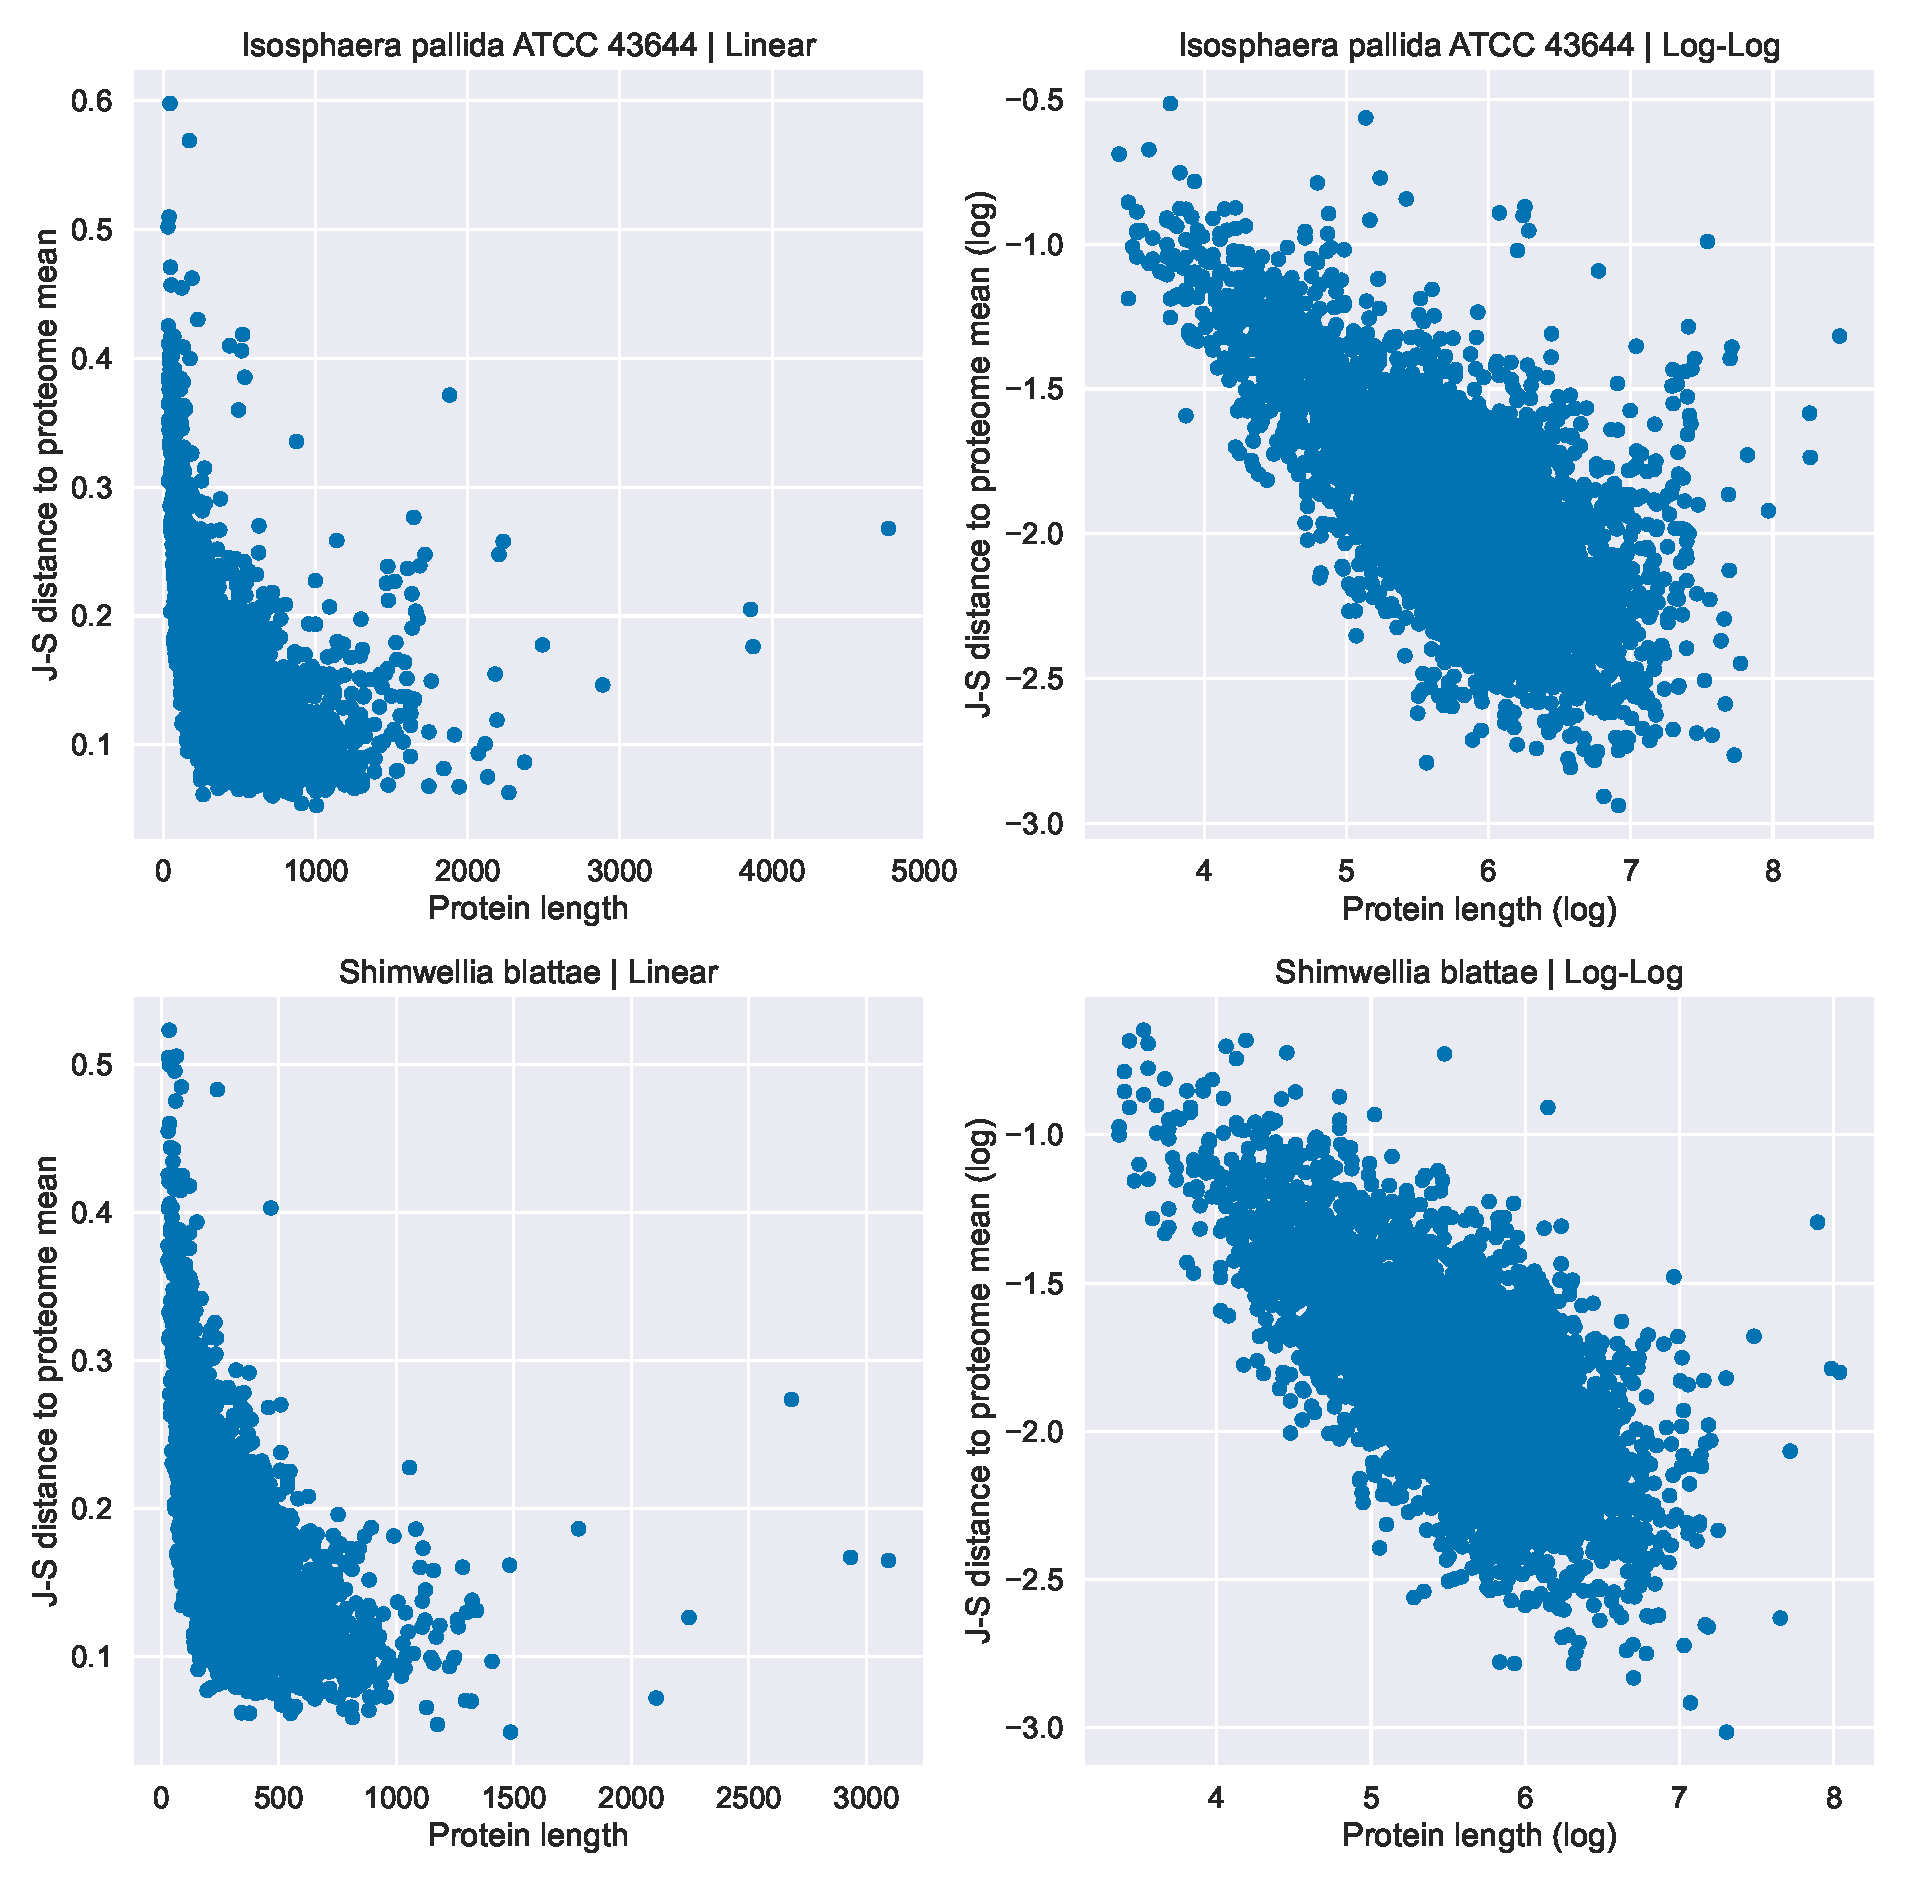
\includegraphics[scale = .55]{length_vs_distance.eps}
\caption{Length versus Jensen-Shannon distance to proteome mean for two organisms. The log-log plot on the right makes the relationship clear.}
\label{fig:length_vs_distance}
\end{figure}

\section{Average protein lengths in top results}

Figure~\ref{fig:average_protein_length} shows the average protein length for 3 different categories of proteins across all of the complete genomes in our dataset:
%
\begin{itemize}
  \item Top 50: proteins appearing at the top of our result set (i.e. tRNA synthetases \& co)
  \item Bottom 50: proteins appearing at the bottom of our result set (i.e. Ribosomal proteins \& co)
  \item Control: 50 proteins sampled randomly in each assembly.
\end{itemize}
%
Top results tend to have a long amino acid chain on average, although the distribution is still covering a lot of ground. Bottom results (i.e. mostly ribosomal proteins, known to be small) have a much smaller average length than the control.

\begin{figure}[!htb]
\hspace*{-1.7cm}
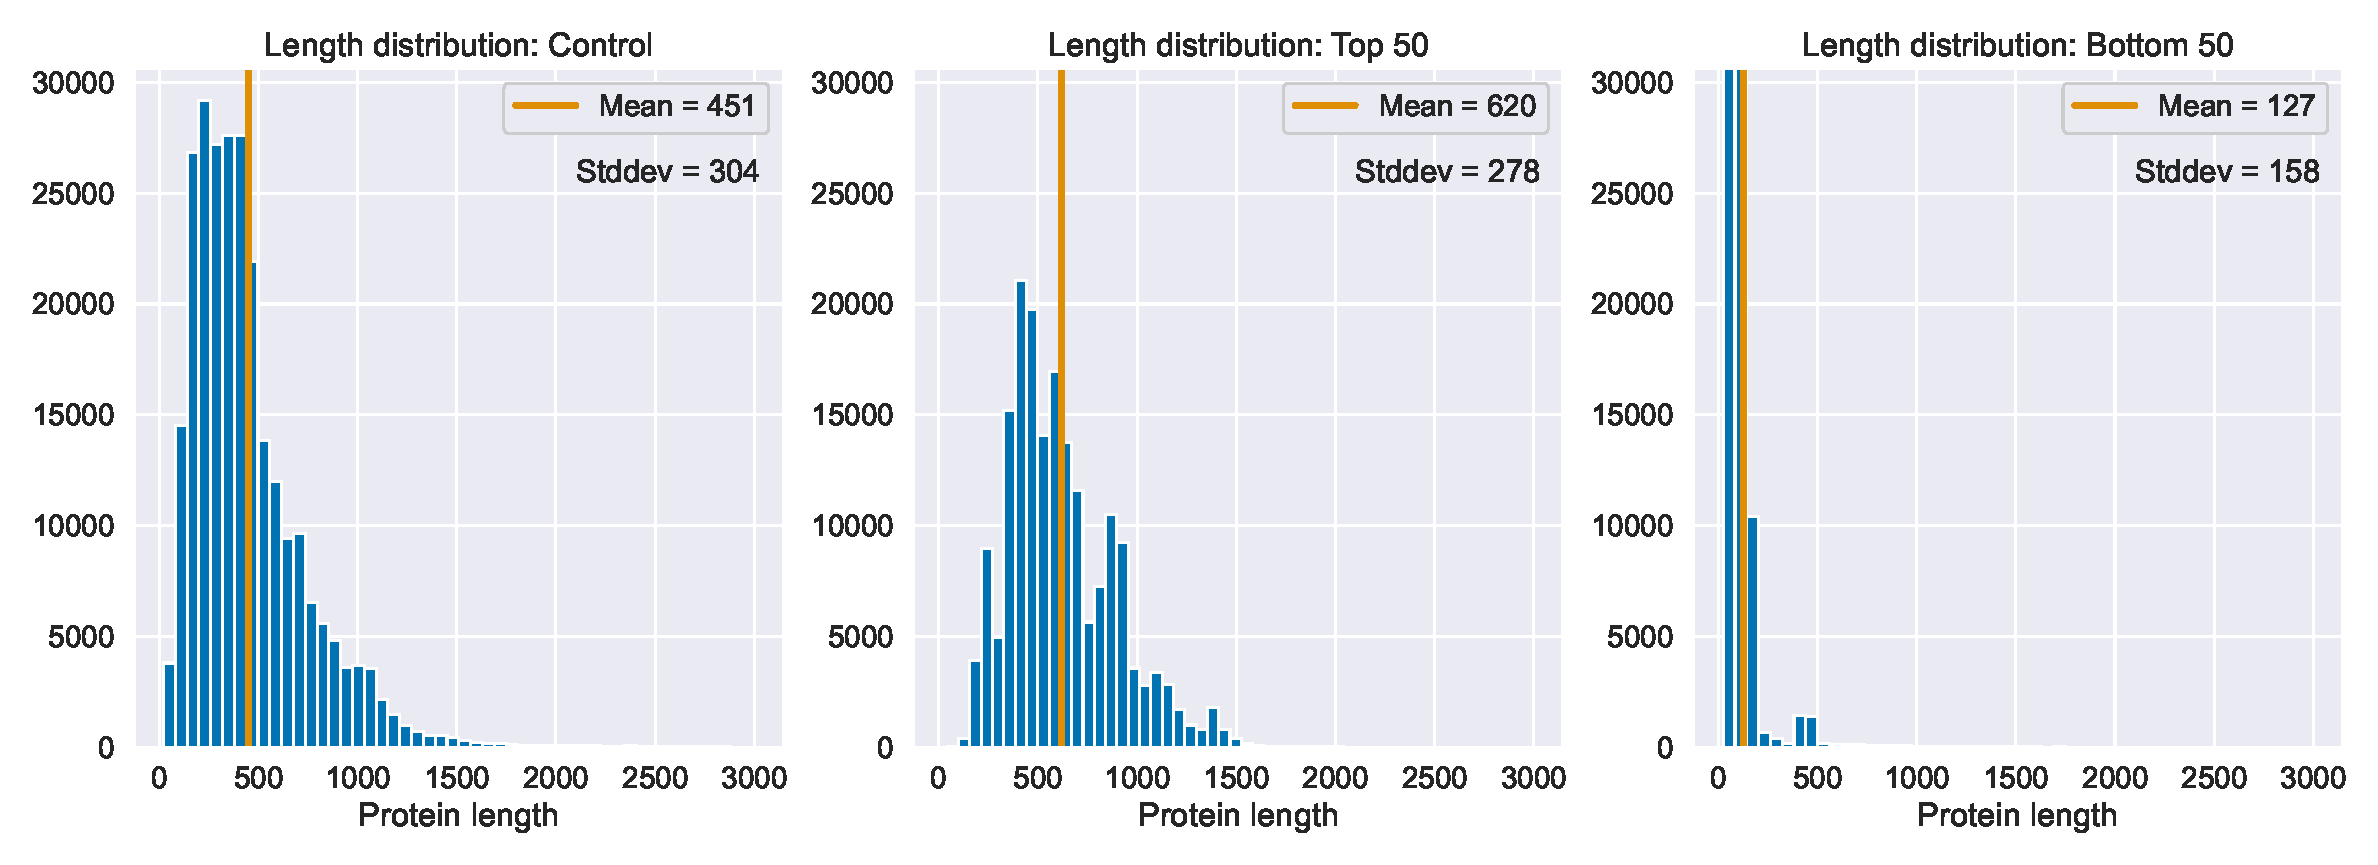
\includegraphics[scale = .45]{average_protein_length.eps}
\caption{Average protein length in three categories of proteins: Control (randomly selected), Top 50 \& Bottom 50 (first and last 50 proteins from our analysis results, respectively)}
\label{fig:average_protein_length}
\end{figure}

\pagebreak

\section{Modeling the relationship}

Next I looked at modeling the relationship between length and distance, in order to compare the goodness of fit between the three groups of proteins defined above (Top 50, Bottom 50, Control).
\newline
\newline
I fit a linear model (from the data projected in log-log space) for each assembly and compared the goodness of fit ($R^2$) overall and in each of the 3 categories. An example of fit is shown in figure~\ref{fig:length_fit_example} and the goodness of fit comparison is plotted in figure~\ref{fig:r_squared_comparison}.
\newline
\newline
On average, length is a fair predictor of distance ($R^2 = 0.45$). However, when selecting a subset of proteins from the top (e.g. tRNA synt) or bottom (e.g. ribosomal proteins) the average fit drops significantly (to sub zero values, i.e. no fit).
\newline
\newline
Note that sample size has an impact on $R^2$, which probably explains the difference between control (similar sample size as top \& bottom) and overall (larger sample).

\section{Discussion}

Length is a decent predictor of distance on average (larger proteins are often more similar to the proteome distribution), however when looking carefully at out top results, the goodness of fit falls dramatically.
\newline
\newline
We can safely conclude that length is not a meaningful confounder.

\begin{figure}[!htb]
\hspace*{-2cm}
\includegraphics[scale = .5]{length_fit_example.pdf}
\caption{Fit of the relationship between length and distance for one example.}
\label{fig:length_fit_example}
\end{figure}

\begin{figure}[!htb]
\hspace*{-1.8cm}
\includegraphics[scale = .65]{r_squared_comparison.eps}
\caption{Average goodness of fit across all individual models (one per assembly) in different protein categories (top vs bottom vs control vs overall).}
\label{fig:r_squared_comparison}
\end{figure}

\end{document}
